\documentclass[12pt,a4paper,english,twoside]{book}
\usepackage[english]{babel}
\usepackage[T1]{fontenc}
\usepackage[utf8]{inputenc}
\usepackage{amsfonts}
\usepackage{amsmath}
\usepackage{latexsym}
\usepackage{amssymb}
\usepackage{epsfig}
\usepackage{moreverb}
\usepackage{rotating}
%\usepackage{enumerate}%
\usepackage{graphics, graphicx,wrapfig}
\usepackage{fancybox}
\usepackage{picinpar,varioref,floatflt}
\usepackage{ae}
\usepackage{longtable}
\usepackage{textcomp}
\usepackage{float}
\usepackage{url}
\usepackage{listings}

\graphicspath{{images/}}

\setlength{\fboxsep}{3pt}%
\setlength{\fboxrule}{1pt}%
\setcounter{section}{1}

%%%%%%%%%%%%%%%%%%%%%%%%%%%%%%%%%%%%%%%%%%%%%%%%%%

% Define the language of the diploma thesis
\selectlanguage{english}
%\selectlanguage{german}

% Define available list stylings

\usepackage{color}
\definecolor{gray}{rgb}{0.4,0.4,0.4}
\definecolor{darkblue}{rgb}{0.0,0.0,0.6}
\definecolor{cyan}{rgb}{0.0,0.6,0.6}

\lstset{ % General setup for the package
	language=Perl,
	basicstyle=\small\sffamily,
	numbers=left,
 	numberstyle=\tiny,
	frame=tb,
	tabsize=4,
	columns=fixed,
	showstringspaces=false,
	showtabs=false,
	keepspaces,
	commentstyle=\color{red},
	keywordstyle=\color{blue}
}

% supress chapter names %
\renewcommand{\chaptername}

% supress numbering %
\renewcommand{\thechapter}{}

\renewcommand{\Link}[3][]{}

\begin{document}

\section*{Registration}
\label{sec:registration}

\subsection*{Step 1}
The reimbursement-tool is connected to the UZH-IFI LDAP server. This allows employees of the IFI department to use their existing login-credentials provided by the University of Zurich.\newline
On the initial login the user needs to pass a two-step registration process. See figure \ref{fig:registration-step01} for the first step. Here, the user needs to input two values:
\begin{itemize}
    \item UZH personnel number is the employee number, written on the employment card. It is of the form \textit{01-123-456}. Enter the number without the leading 0 and hyphens; i.e. \textit{123456}.
    \item UZH phone number is the personnel phone number of the employee. Please enter it in the form \textit{0441234567}.
\end{itemize}\newpage

Furthermore the user can select his preferred language. However, the language will be automatically determined based on the browser language settings.\par
An account can also be deactivated, so that the user cannot participate actively in the reimbursement-process.

\begin{figure}[H]
    \centering
    \fbox{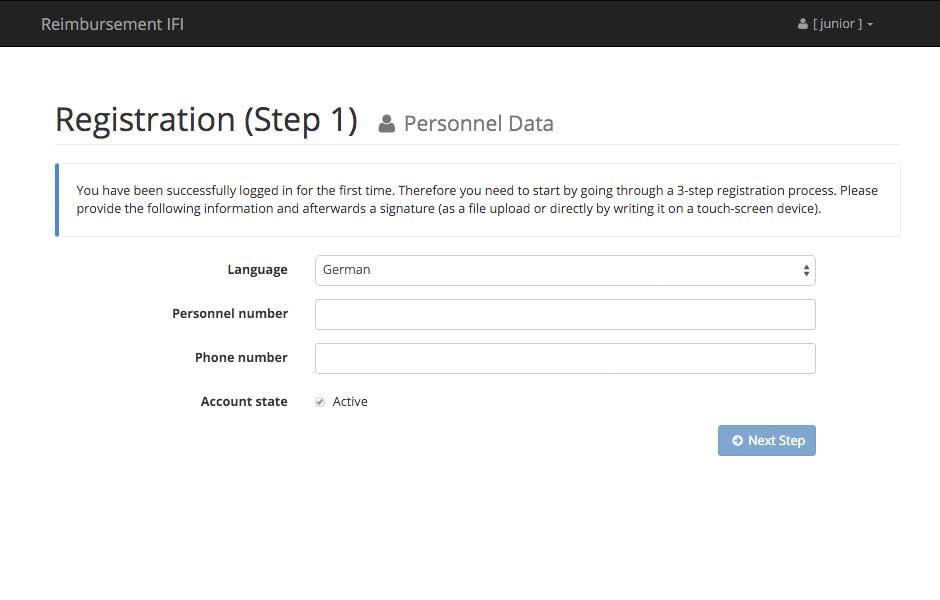
\includegraphics[width=0.80\textwidth]{registration-step01.jpg}}
    \caption{Registration step one: Capture personnel data}
    \label{fig:registration-step01}
\end{figure}

\subsection*{Step 2}
On figure \ref{fig:registration-step02} the user needs to add his handwritten signature either by uploading an image or capture it using a third party touchscreen device, i.e. a smart phone. This signature is required later on to stamp it onto the generated Pdf document containing all receipts.

\begin{figure}[H]
    \centering
    \fbox{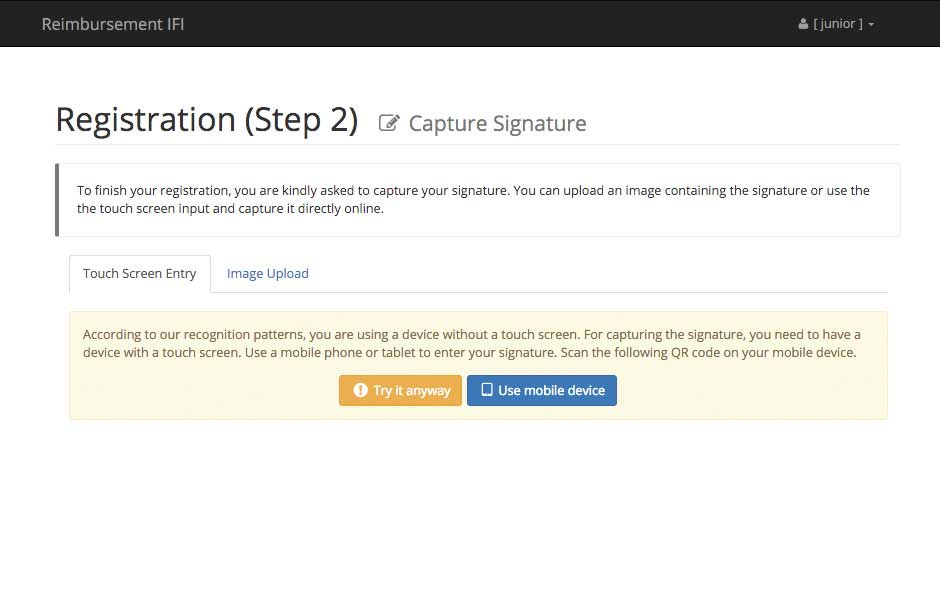
\includegraphics[width=0.80\textwidth]{registration-step02.jpg}}
    \caption{Registration step two: Capture signature}
    \label{fig:registration-step02}
\end{figure}

After completing the registration process, the captured information and signature can always be edited by navigation to the \textbf{Settings} on the navigation bar.

\section*{Expenses}

An expense is an entity captured by a \textit{Registered user}. Every expense is defined by an \textbf{SAP description} that will be visual in SAP. An expense consists of 1 to 15 receipts.

The \textit{Registered user} has to create an expense, add receipts to it and submit it to a \textit{Manager}. The system selects the respective \textit{Manager} automatically given that is defined. The \textit{Manager} will check the expense for correctness, add the corresponding projects and submit it to be approved by the \textit{Finance management}. For a detailed description of the overall reimbursement-process refer to section \ref{sec:process}.

\subsection*{Create Expense}

To create an expense, the user needs to navigate to the \textbf{Dashboard} and click on the button \textbf{Create new Expense}. A modal-window will appear to enter the \textbf{SAP description}. Once it is entered correctly and the user clicked \textbf{Next} an empty expense will be created. The user can start with adding receipts (see figure \ref{fig:expensesitems-overview}).

\begin{figure}[H]
    \centering
    \fbox{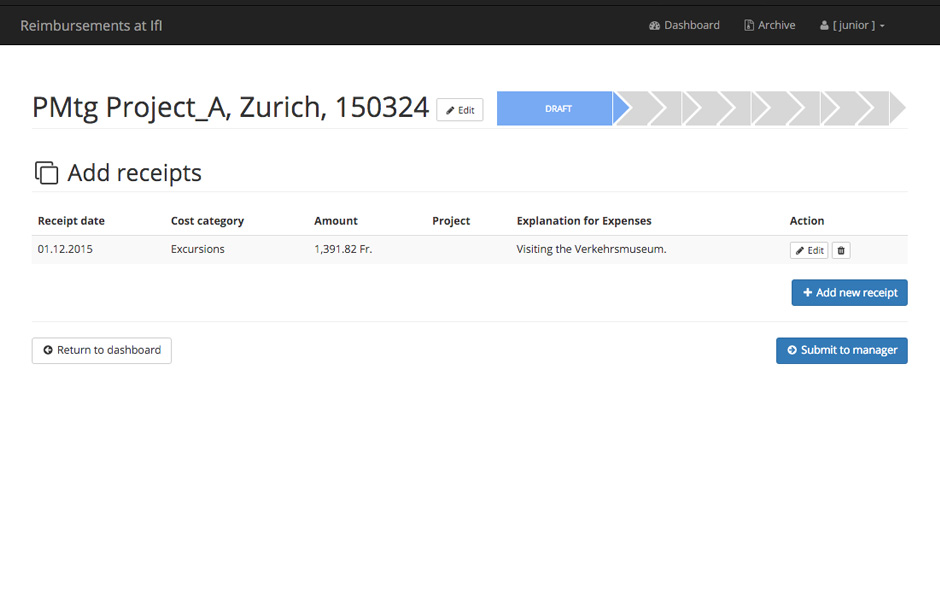
\includegraphics[width=0.80\textwidth]{expensesItems-overview.jpg}}
    \caption{Expense-View: Overview}
    \label{fig:expensesitems-overview}
\end{figure}

On the top left-hand side the \textbf{SAP description} is added. The small \textbf{Edit} button on the right can be used for editing. On the top right-hand side the current process step and the unprocessed steps of the expense are visualized. This process bar always indicates the current state of the expense.\newline
Further the user can add, edit and remove receipts. To add a new receipt the user needs to click on the button \textbf{Add new Receipt}. See section \ref{sec:addreceipt} for details. \newline
Existing receipts can be edited and removed by clicking on the respective buttons.


\subsection*{Receipt}
\label{sec:addreceipt}
By adding a new receipt or editing an existing one, the user needs to fill out the following mandatory fields:
\begin{itemize}
    \item \textbf{Receipt date} will be used to calculate the correct exchange rate if a foreign currency is selected.
    \item \textbf{Cost category} selected based on a pre-defined list of available cost categories.
    \item Original and calculated amount based on the exchange rate. The rate used in the system is based on the market rate plus a 2\% variation immunity.

    \item The \textbf{project assignment} is added by a user with role \textit{Manager} or \textit{Department manager}.
    \item A short \textbf{explanation} that describes the purpose of the receipt.
    \item \textbf{Receipt attachment} consists of an uploaded document that verifies the input information like receipt date, price and currency.
\end{itemize}

See figure \ref{fig:expenses-add01}.


\begin{figure}[H]
    \centering
    \fbox{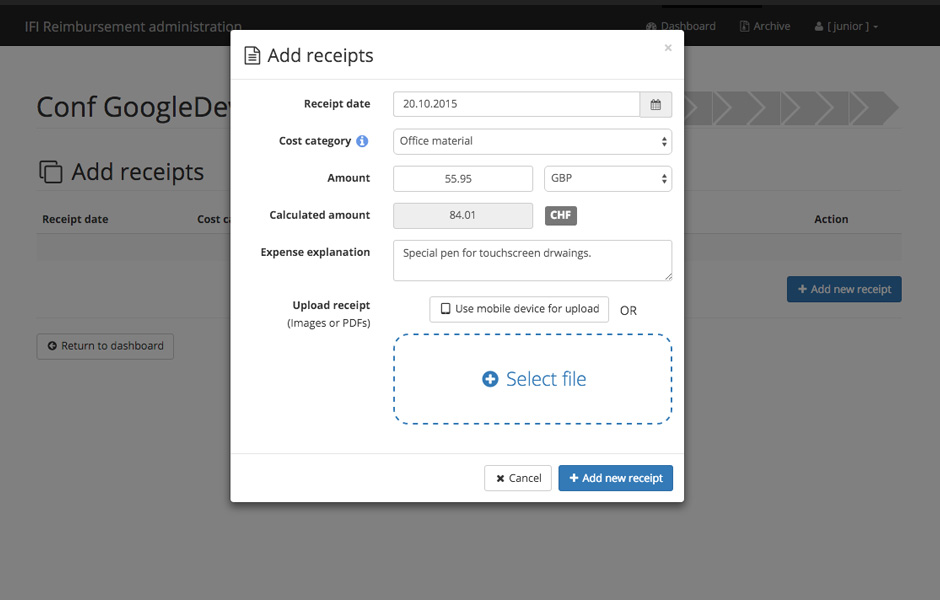
\includegraphics[width=0.80\textwidth]{expenses-add01.jpg}}
    \caption{Expense: Add new receipt}
    \label{fig:expenses-add01}
\end{figure}

\subsection*{Assign Expense to Manager}
If all receipts are captured, the expense will be submitted to a \textit{Manager}. Once it is submitted, it cannot be edited by the \textit{Creator} anymore.

\subsection*{Sign document}
\label{sec:signing}
The signing is required for the generation of the Pdf that contains all of the captured receipts of the expense. This Pdf uses the signatures of the respective \textit{Creator}, \textit{Manager} and \textit{Finance management} to proof their acceptance of the expense and the captured receipts. During the signing process the user will be prompted to select his preferred signing method (see figure 3.5). The two different types available will be explained in detail:
\begin{itemize}
    \item A \textbf{Digital signature} ensure the authenticity of the signer. Any changes made to the document after it has been signed will invalidate the signature. To use it the user has to provide his private key to successfully sign the document.
    \item \textbf{Electronic signature} does not ensure the authenticity of the signer. Anyone can theoretically make changes on the document after it has been signed without the signature become invalid. The handwritten signature captured at the registration (see section \ref{sec:registration}) will be stamped on the Pdf document.
\end{itemize}

\begin{figure}[H]
    \centering
    \fbox{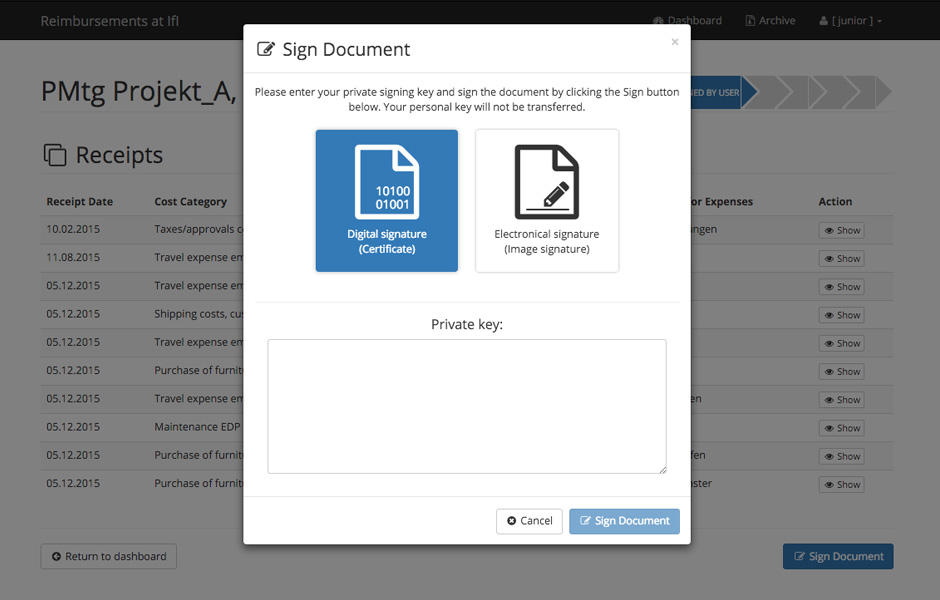
\includegraphics[width=0.80\textwidth]{expenses-sign.jpg}}
    \caption{Expense: Sign document}
    \label{fig:expense-sign}
\end{figure}

Please note, that if a signing method has been selected all subsequent signers, like \textit{Manager} and \textit{Finance management} have to apply the same method.


\section*{User roles}
\label{user-roles}

Every user that exists in the LDAP of the University of Zurich is capable to login to the system. He can use the same user name and password that he uses for the other University of Zurich services for login.

The reimbursement-tool provides different user roles. The roles on the reimbursement-tool are mapped with the LDAP user roles of the University of Zurich. So a user who is defined as professor for a specific group on the LDAP will be the manager for all users of this group. The reimbursement-tool provides the following roles:

\begin{itemize}
    \item \textbf{Unregistered user} are users, who are authorized to login the reimbursement-tool but have not yet completed the registration process, see section \ref{sec:registration}.
    \item \textbf{Registered user / User} passed the registration process. He can access the reimbursement-tool and create and manage his created expenses. He has one of the following roles:

    \begin{itemize}
        \item \textbf{Creator} iis authorized to create, edit and print expenses as long as they are in DRAFT state. He's the initial creator of an expense.

        \item \textbf{Manager / Professor} are authorized to reject, accept and edit expenses as long as they are assigned to him.

        \item \textbf{Department manager} has the same authorizations as the \textit{Manager}. If a \textit{Manager} is outreach, his assignments will be forwarded to the respective \textit{Department manager}.

        \item \textbf{Finance management} is authorized to reject, accept and edit expenses once they have been accepted by a \textit{Manager} or \textit{Department manager}. Furthermore they can manage the available cost categories and search for expenses.

        \item \textbf{Head of institute} has the same authorizations as the \textit{Manager}. In contrast to the \textit{Department manager} there exists only one \textit{Head of institute}.
    \end{itemize}
\end{itemize}

\section*{Guest view}
The guest view allows users to retrieve expenses without the need of a user with role \textit{Registered user} for the reimbursement-tool. They can open the guest view using a special URL. It is provided on every printed expense document (see figure \ref{fig:pdf-web}). The URL is located on the lower right side of the page in form of a QR-Code and an URL. So that the user can either scan the QR-Code or typewrite the URL in a browser window and he'll get access to the respective expense. \newline
The expense can be accessed using the URL provided for the prospective 6 months of the creation of the pdf.

\begin{figure}[H]
    \centering
    \fbox{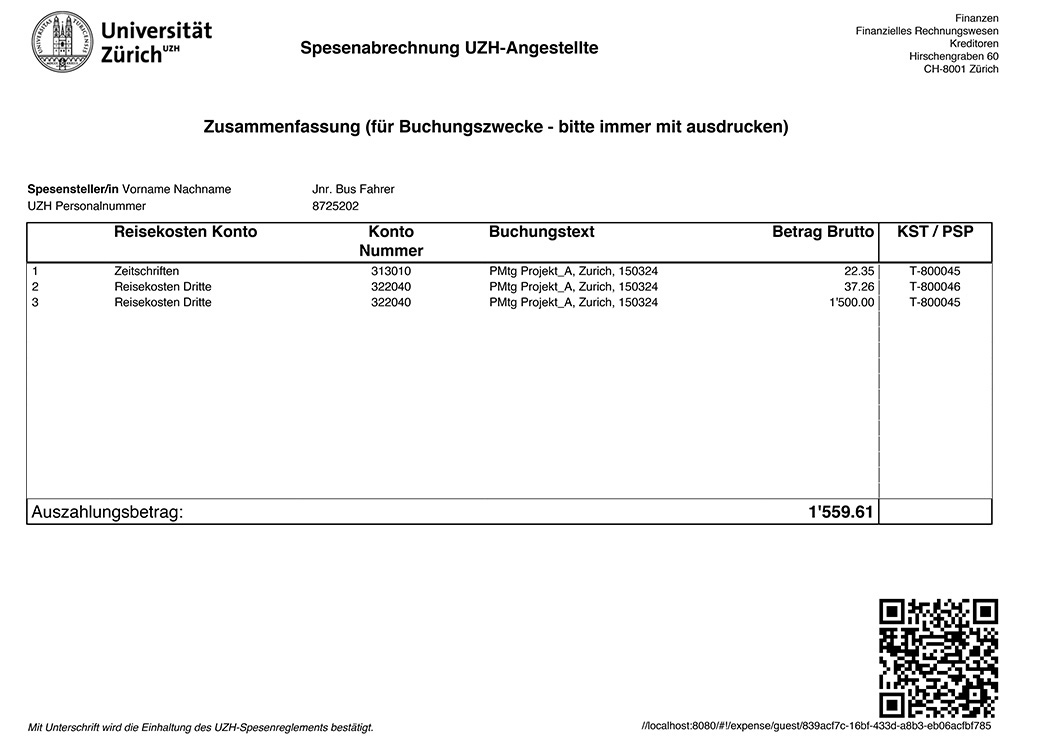
\includegraphics[width=0.80\textwidth]{pdf-web.jpg}}
    \caption{Administration: Pdf guest view link}
    \label{fig:pdf-web}
\end{figure}

\section*{Cost categories}

The existing cost categories of the reimbursement-tool can be edited and deactivated by the \textit{Finance management}. Furthermore a new cost category can be created by providing the German and English translation for it. See figure \ref{fig:admin-costcategories}.

\begin{figure}[H]
    \centering
    \fbox{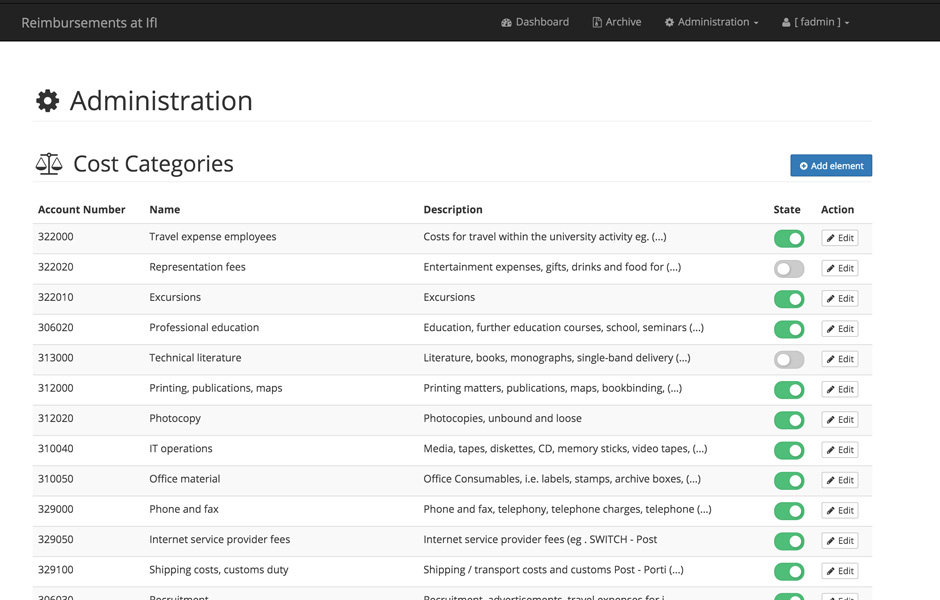
\includegraphics[width=0.80\textwidth]{admin-costcategories.jpg}}
    \caption{Administration: Cost categories}
    \label{fig:admin-costcategories}
\end{figure}

\section*{Retrieve Expenses}
\subsection*{Search for Expenses}

For the \textit{Finance management} users a sophisticated search interface for expenses exist; the \textit{Admin Pool Search} (see figure \ref{fig:admin-search}). The search result will be limited by the following values:

\begin{itemize}
    \item Specify the date range the expense has been created.
    \item Last name of the expense applicant.
    \item The permission / role of the applicant.
    \item The current state of the expense.
    \item Based on the selected cost category of the receipt.
    \item The accounting description (similar to the SAP description).
\end{itemize}

\begin{figure}[H]
    \centering
    \fbox{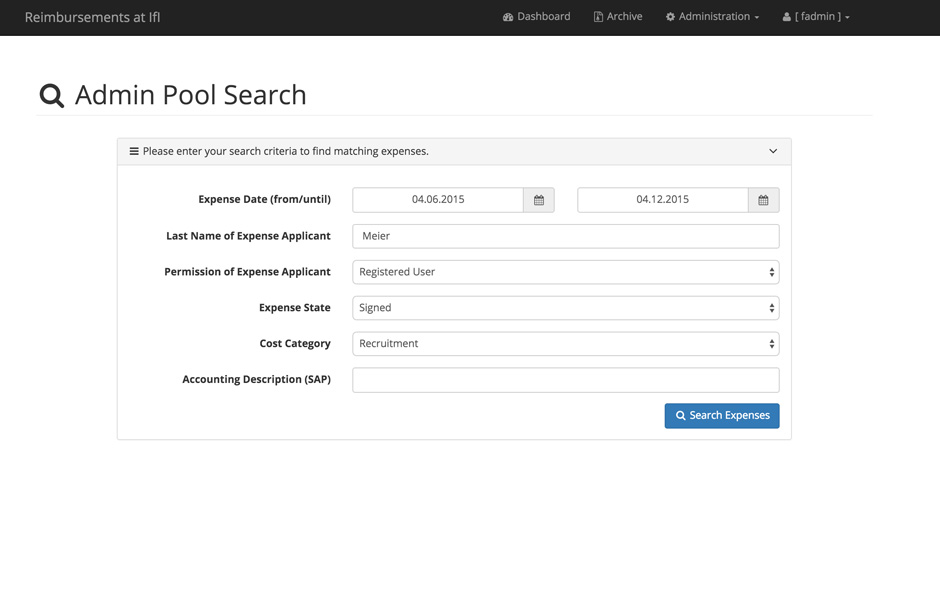
\includegraphics[width=0.80\textwidth]{admin-search.jpg}}
    \caption{Administration: Search for \textit{Expenses}}
    \label{fig:admin-search}
\end{figure}

The \textit{Finance management} users are authorized to execute specific actions to change the expense state:
\begin{itemize}
\item \textbf{Reassign}: If the expense has been already printed by the user, it can be reassigned to a \textit{Finance management} user.
\item \textbf{Reset}: has mistakenly submitted the expense, it can be reset and assigned back to him.
\end{itemize}

\subsection*{Archive}
Besides the \textit{Admin Pool Search} there exists an archive page for all users. The archive provides a list of all expenses in \textit{PRINTED} state that the current, logged-in user has created.

\subsection*{Analytics}
The reimbursement-tool provides an analytics-view for the \textit{Finance management}. It should help to empower their knowledge about the overall amount of the captured expenses, rate of printed expenses as well as the actual state-distribution among the expenses.


\section*{Expense process}
\label{sec:process}

The entire process is basically divided into three iterations. The \textbf{1. iteration}; expense creation and confirmation, \textbf{2. iteration}; the expense signing, \textbf{3. iteration}; print and carry the documents to the \textit{Finance management} of the University of Zurich.\newline
Expense date, cost category, amount, explanation and attachment will be captured by the user, who is the expense \textit{Creator}. As soon as he's done with capturing and submitting the expense, it'll be assigned to the \textit{Manager}. The \textit{Manager} reviews the expense, adds the respective projects and assigns the expense to the next instance for review; the \textit{Finance management}. If they are satisfied, they submit it and the expense moves into the second iteration; the signing. For more detailed information containing the signing refer to section \ref{sec:signing}.\newline

\begin{figure}[H]
    \centering
    \fbox{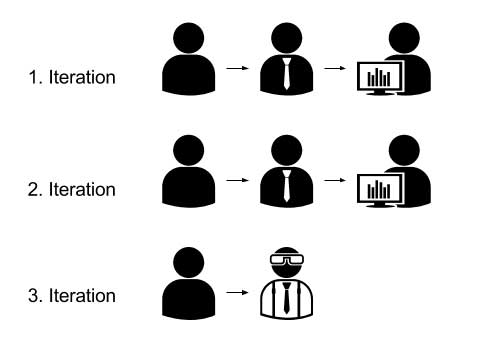
\includegraphics[width=0.80\textwidth]{expense-process.jpg}}
    \caption{Expense: Process of expense creation}
    \label{fig:expense-process}
\end{figure}

After the signing is completed by all instances. The expense will be available to print by the \textit{Creator}. As soon as all the documents are printed, they need to be carried to a \textit{Finance management} user for further processing. The \textit{Finance management} will send all relevant documents to the Finance Administration of the University of Zurich. This action completes the process.


\end{document}
